\subsection{Photons}
\label{sec:photons}

The kinematic requirements applied on the photons, after the diphoton candidates have passed through the event pre-selection (see Section ~\ref{sec:trigger}), is analogous to the ones used in the SM $\Hgg$ analysis. The selection is as follows:
\begin{itemize}
\item Leading photon $E_{T} > 30 \GeV$, trailing photon $E_{T}>20 \GeV$;
\item Leading photon $E_{T}/\Mgg > 1/3$, trailing photon $E_{T}/\Mgg > 1/4$;
\item $100 < \Mgg < 180 \GeV$.
\end{itemize}
Additionally, a photon identification requirement is applied to the photons.

In the 13\TeV run of 2016 we have at least three different identification algorithms for
photons:
\begin{itemize}
\item General purpose cut-based ID developed by the CMS EGamma
  group~\cite{PhotonCutBasedID-twiki}. The ID makes use only of a few variables: H/E,
  $\sieie$ and isolation. This type of ID was used in Run-I analysis.
\item General purpose MVA ID developed within the EGamma
  group~\cite{PhotonMvaID-twiki}. It utilizes the information from many shower shape
  variables at ECAL, as well as isolation information.
\item MVA ID developed by the $\Hgg$ search group~\cite{HggMvaID-slides} (ref to be
  updated). It is similar to the one developed in EGamma group, but uses a slightly
  different set of input variables.
\end{itemize}

We have chosen to use the EGM MVA photon ID on this analysis. 
The WP chosen is one that provides $90\%$ signal efficiency for the photon selection (provided centrally). 
The scale factors used to ensure data/MC agreement in the selection efficiency are also applied (provided centrally).
Additionally, an electron veto is applied to avoid background with electrons faking photons (scale factors provided centrally also applied).

=========== OLD ===========

Currently (as of January 2016), the available samples processed by the $\Hgg$ group only have stored 
their own training of the photon MVA ID. 
We have chosen working points that ensure that the resonant low mass samples have 
a $90\%$ efficiency both in the barrel and the endcap ECAL regions. 

\begin{table}[h]
\centering
\begin{tabular} { | c | c | }
\hline
ECAL Region & Hgg MVA Selection \\ \hline
EB & 0.07 \\ \hline
EE & -0.03 \\ \hline
\end{tabular}
\end{table}

Efficiencies of the leading photon to pass the ID criteria, as a function of the photon transverse energy, 
are shown in Figure \ref{fig:Hgg-PhoID-eff}. 
Only photons matched to gen-level prompt photons are used. 


\begin{figure*}[thb]
  \centering
  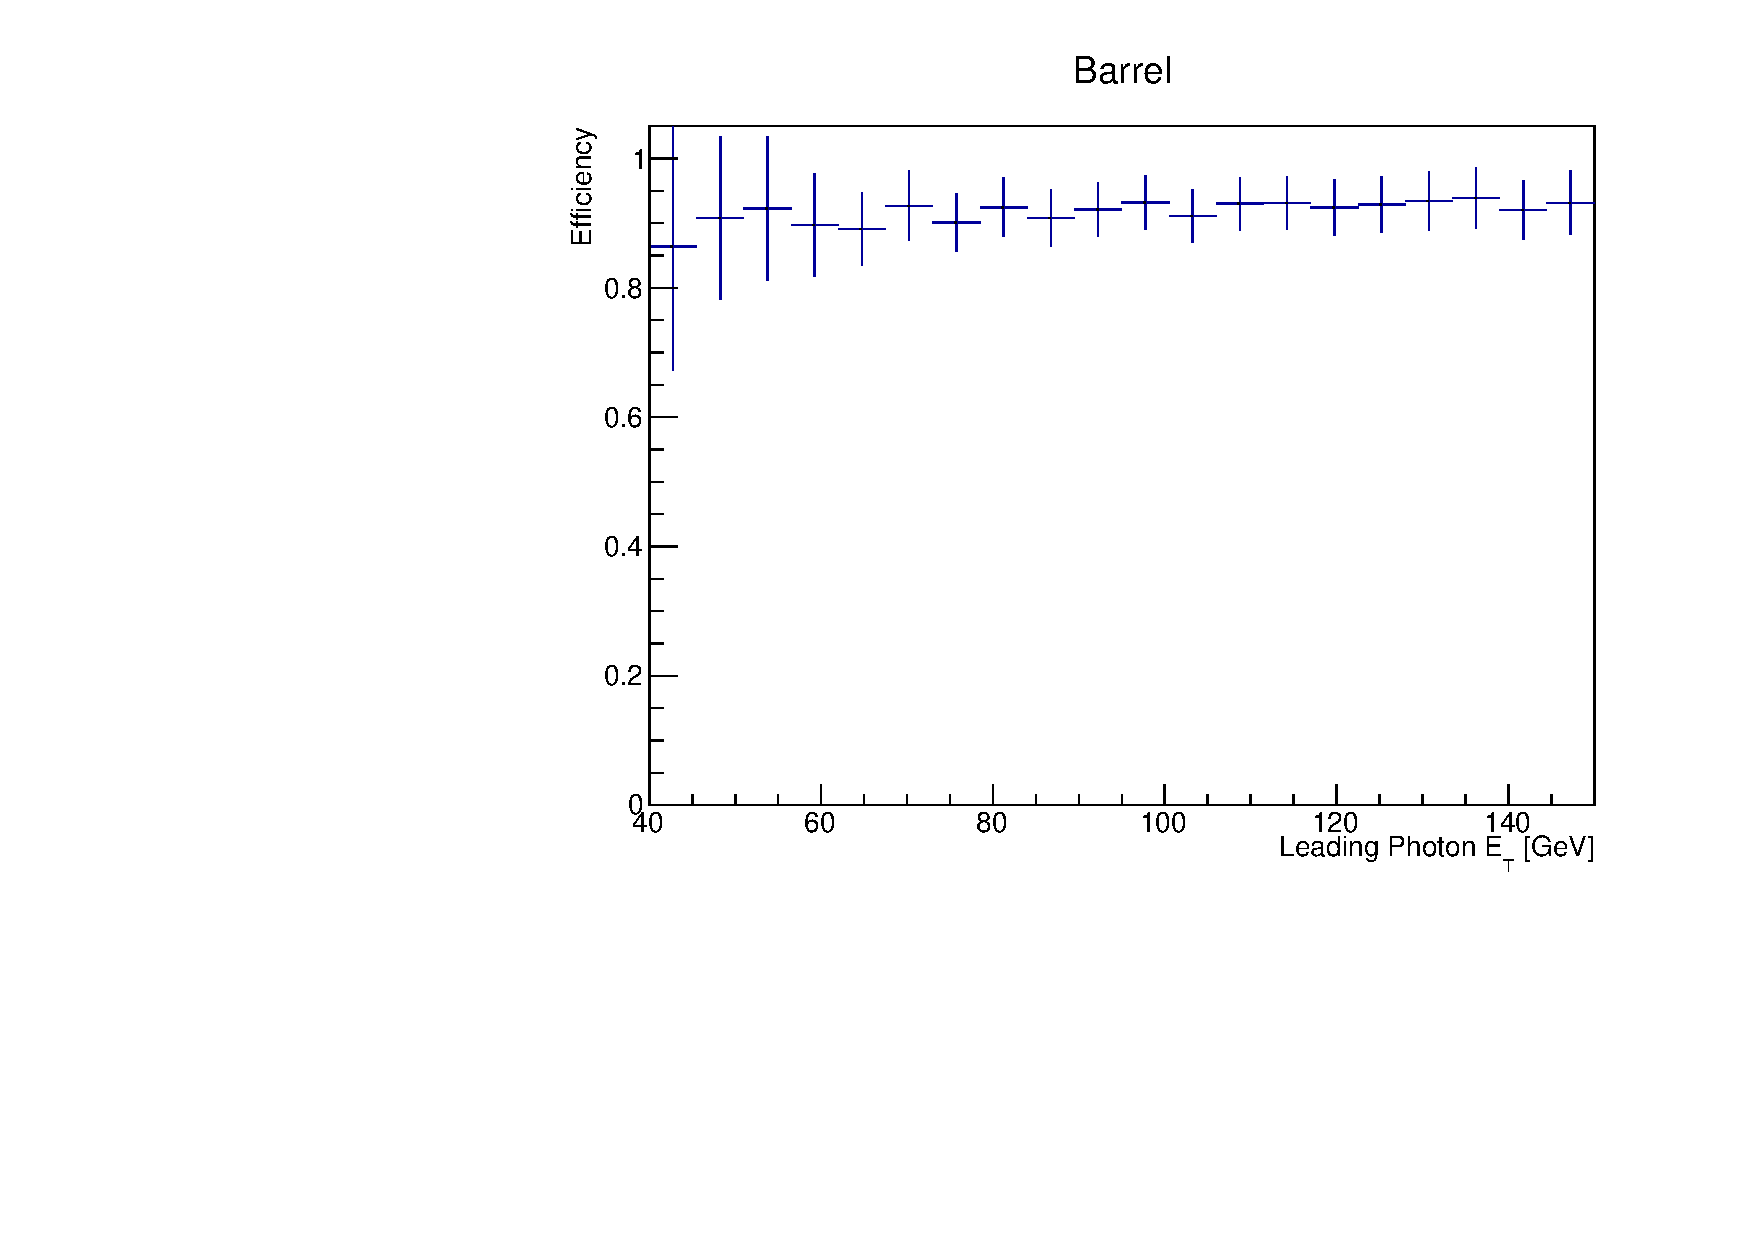
\includegraphics[width=0.45\textwidth]{figures/sec-photons/SMHH_HggMVA_Eff_EB.pdf}\hfil
  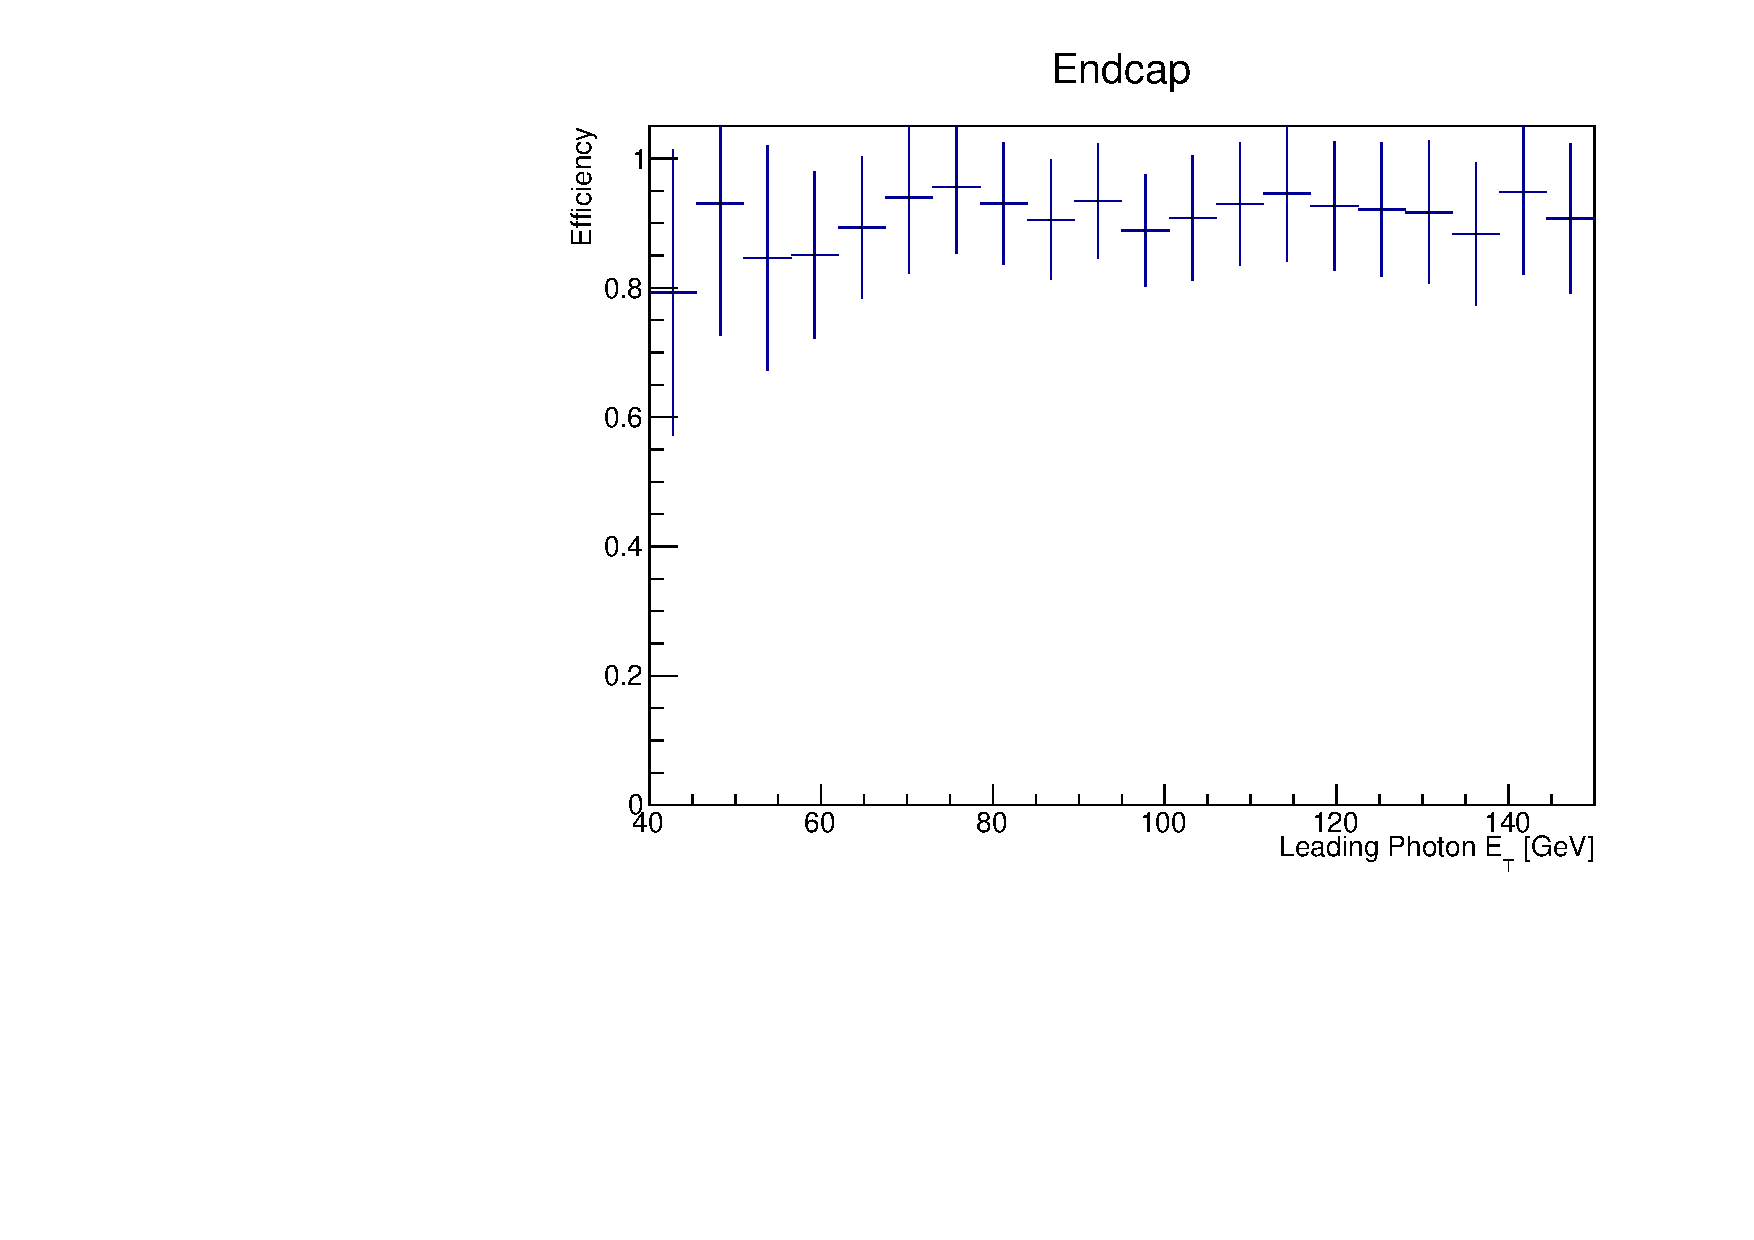
\includegraphics[width=0.45\textwidth]{figures/sec-photons/SMHH_HggMVA_Eff_EE.pdf}\hfil
  \caption{Efficiencies of the leading photon to pass the ID criteria, as a function of the photon transverse energy, 
for photons in the barrel and endcap regions of ECAL. }
  \label{fig:Hgg-PhoID-eff}
\end{figure*}

%We have studied all of those possibilities with MC samples, and for the 2015 data we
%decided to use the MVA ID of EGamma group with \textit{Loose} working point (WP),
%corresponding to 90\% signal selection efficiency.  A brief summary of this study is
%described below.

%The true photons are selected from the $G \to \HH \to \bbgg$ signal MC samples (they are
%required to match the generated level photons within $\Delta R< 0.1$ cone). The fake
%photons are selected from the Double-EM enriched $\gamma$+jet samples (and they must not
%to match to any generated level photon).
%The studied photons must pass the standard photon selection (pre-selection plus kinematic selection).

%Finally, the MVA score is calculated for the selected photons (or an ID decision for the
%cut-based ID).  Figure \ref{fig:phoID-MVA} shows two examples of the MVA output from the
%signal and fake photons. And Figure~\ref{fig:phoID-ROC} shows the ROC curves for the three
%IDs considered, for photons in the Barrel and Endcap. On these curves at a given signal
%efficiency one would prefer to have highest background rejection. From this figure of
%merit the MVA IDs are undoubtedly better than the cut-based ID. While the two MVA IDs have
%very similar performance.

%Note: it is anticipated that for 2016 data-taking the two MVA IDs will merge into one, and we
%will use that.

%\begin{figure*}[thb]
%  \centering
%  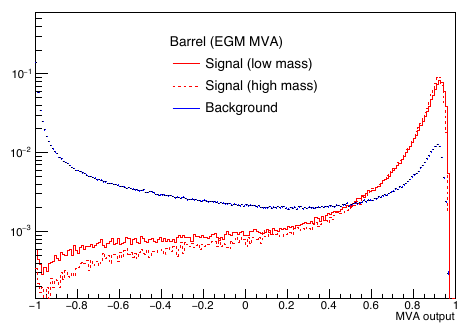
\includegraphics[width=0.45\textwidth]{MVA_output_EGM_Barrel}\hfil
%  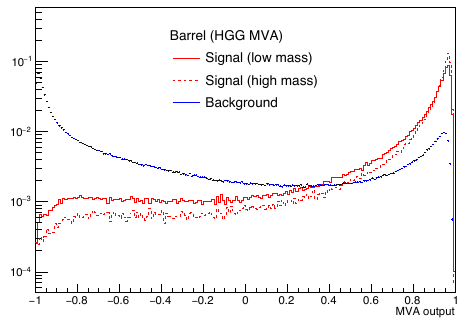
\includegraphics[width=0.45\textwidth]{MVA_output_HGG_Barrel}\hfil
%  \caption{Examples of the MVA ID outputs for the photons in the Barrel. Left: EGamma,
%    right: Hgg.}
%  \label{fig:phoID-MVA}
%\end{figure*}


%\begin{figure*}[thb]
%  \centering
%  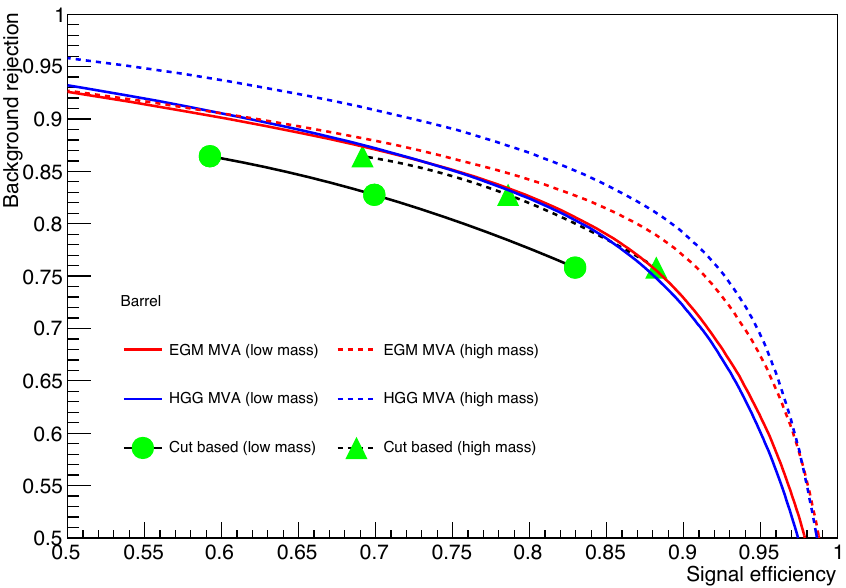
\includegraphics[width=0.45\textwidth]{ming_phoID_EB}\hfil
%  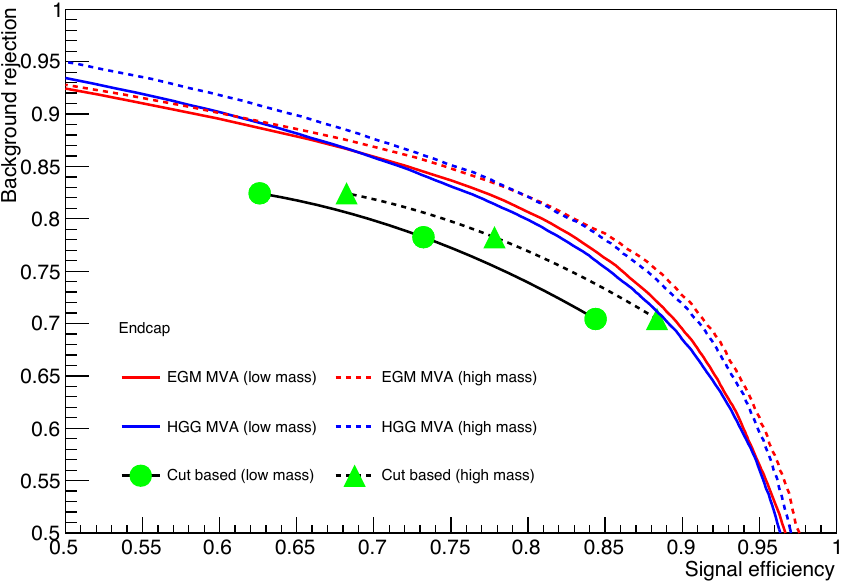
\includegraphics[width=0.45\textwidth]{ming_phoID_EE}\hfil
%  \caption{Photon ID ROC curves}
%  \label{fig:phoID-ROC}
%\end{figure*}

\subsubsection{Fake Photon Control Region}\label{sec:PCR}
A control region is created by selecting diphoton candidates with one photon that passed the ID requirement and one that didn't. All the other selections remain the same, and the procedure to select such diphoton candidate is the same as in the signal region.

This control region is used on the analysis to perform the closure test on the background modeling.

\subsubsection{Vertex}
Inheriting from the main $\Hgg$ analysis, we use the vertex that gives the highest $\Hgg$ vertex MVA score. 
Because there are additional jets in the event, picking picking this vertex has a very small mismatch efficiency. 
Only in less than $0.1\%$ of the events, the chosen vertex is different from the vertex associated to the simulated event. 

\subsubsection{Gain Switch}

Due to the ECAL slew rate issue discovered during the 2016 data taking, we investiaged the fraction of selected events in our blinded signal region with photons that go through gain switches. 
The plots on Figure \ref{fig:gain_switch}  show, in bins of $\tilde{M}_{X}$, the fraction of events with at least one of the photon candidates going through gain switches (to gain 1, gain 6 or both). 
These results show that, for the high mass region, around $20\%$ of our events are affected by gain switches. 
This non-negligible rate means that the analysis needs to use the re-MiniAOD Moriond17 campaign, which has the slew rate effect mitigated.

\begin{figure*}[thb]
  \centering
  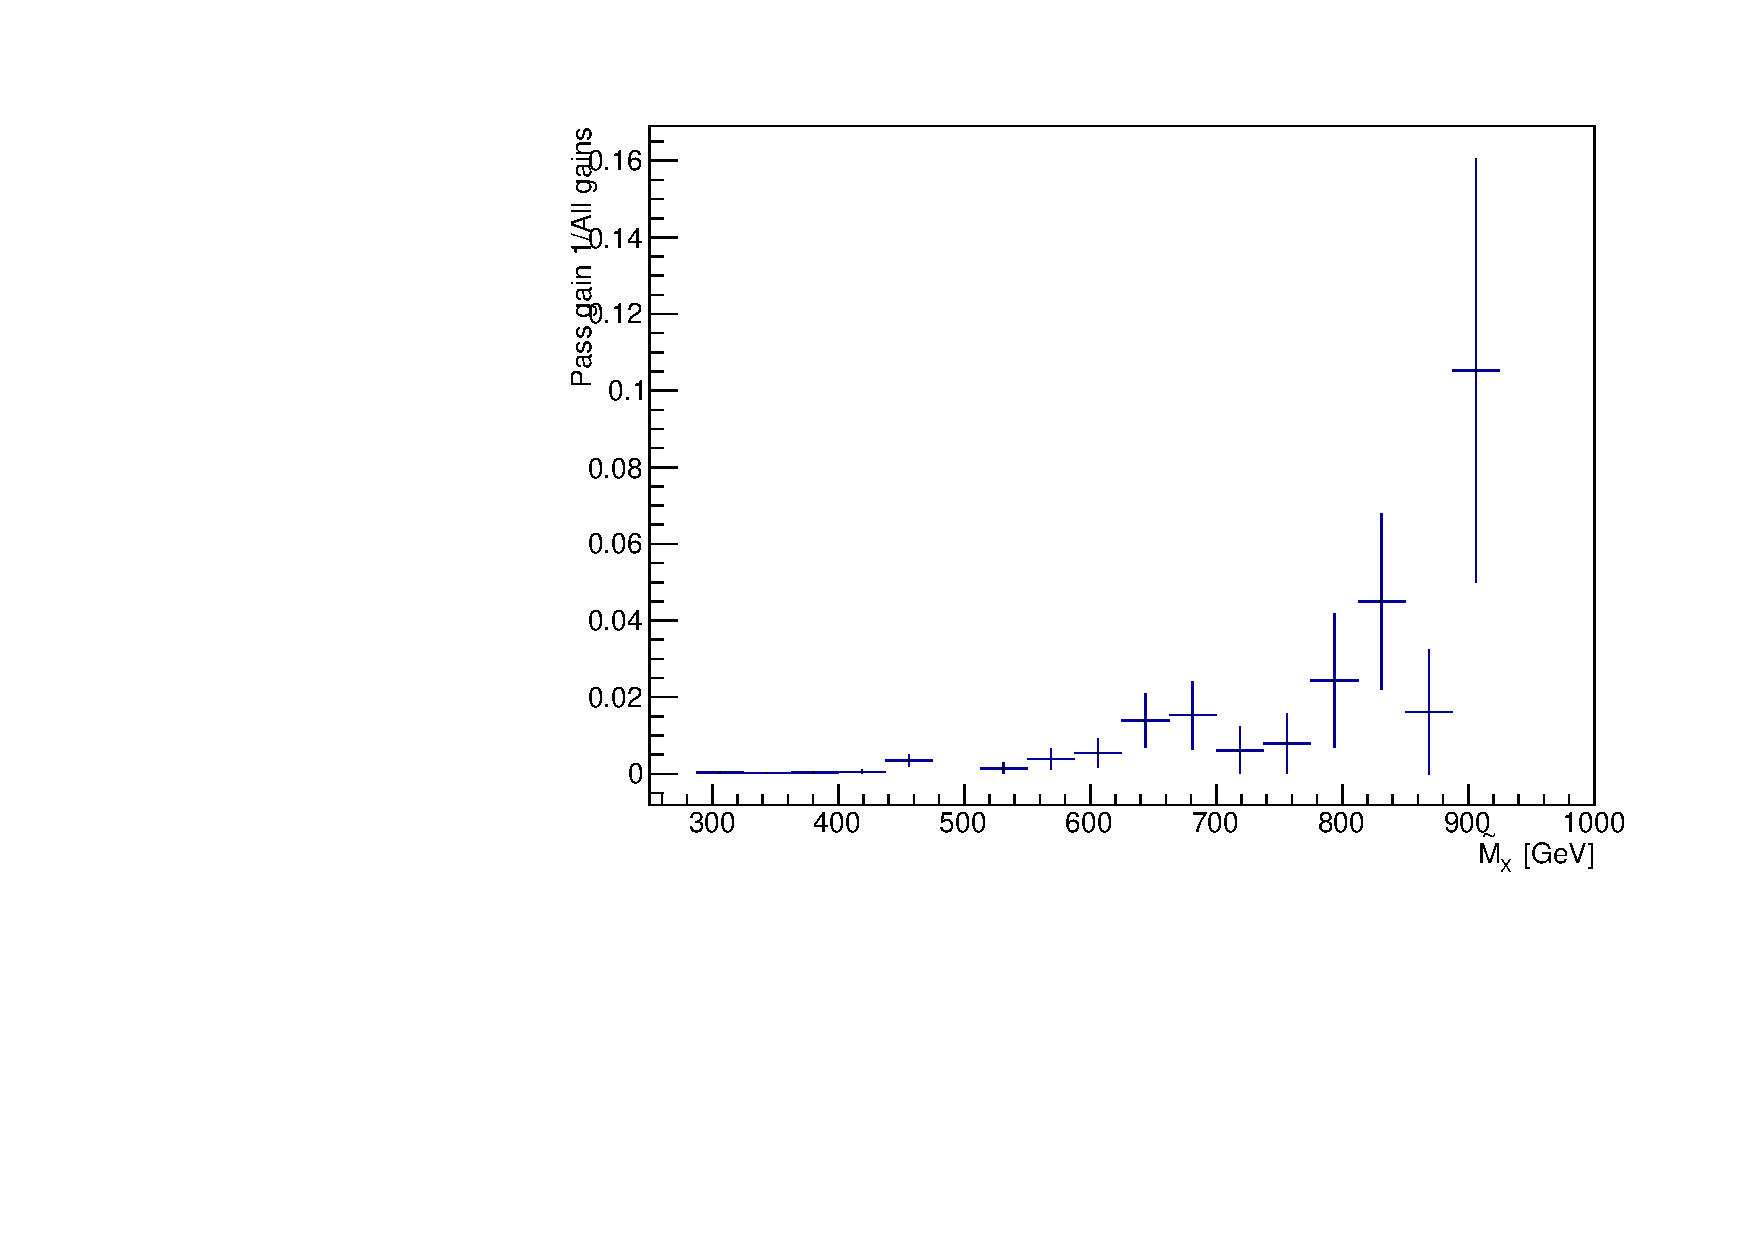
\includegraphics[width=0.3\textwidth]{figures/sec-photons/rg1}\hfil
  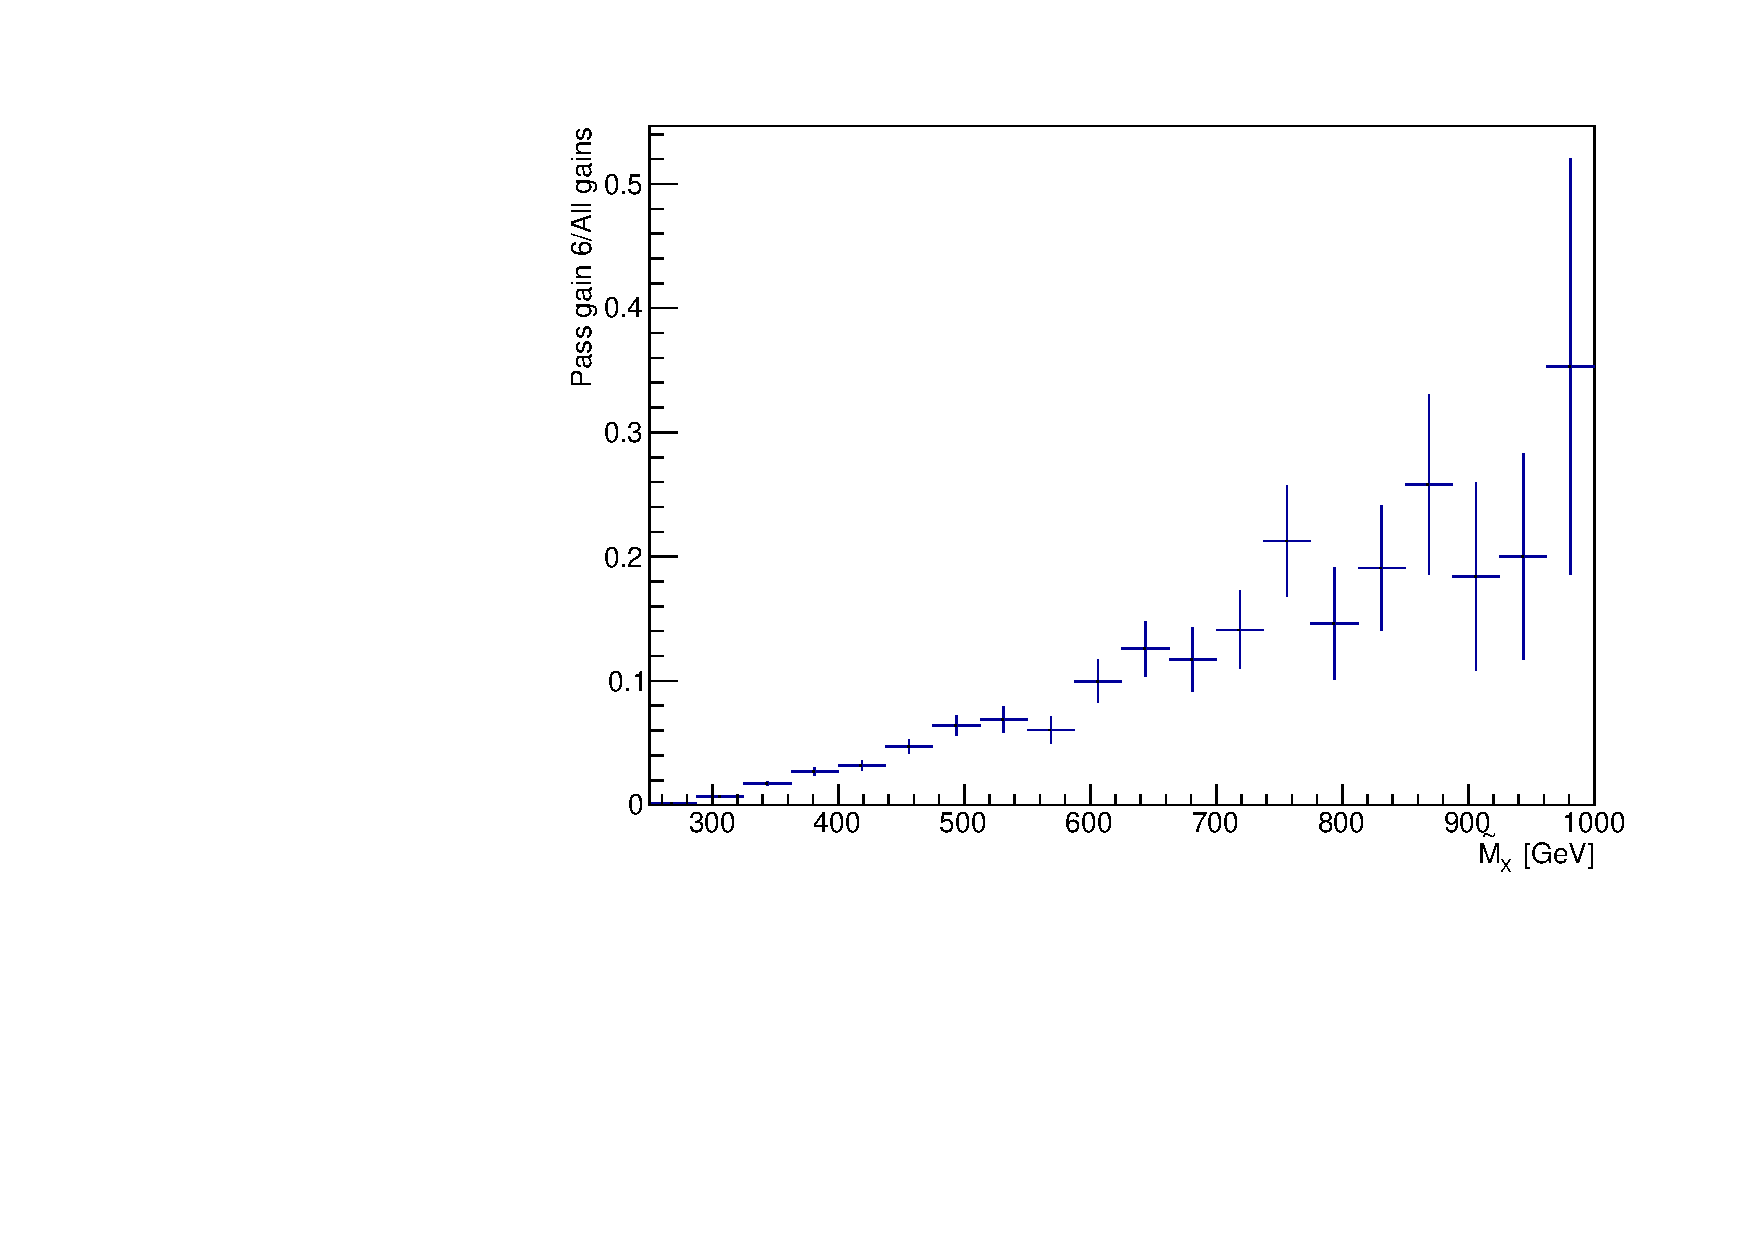
\includegraphics[width=0.3\textwidth]{figures/sec-photons/rg6}\hfil
  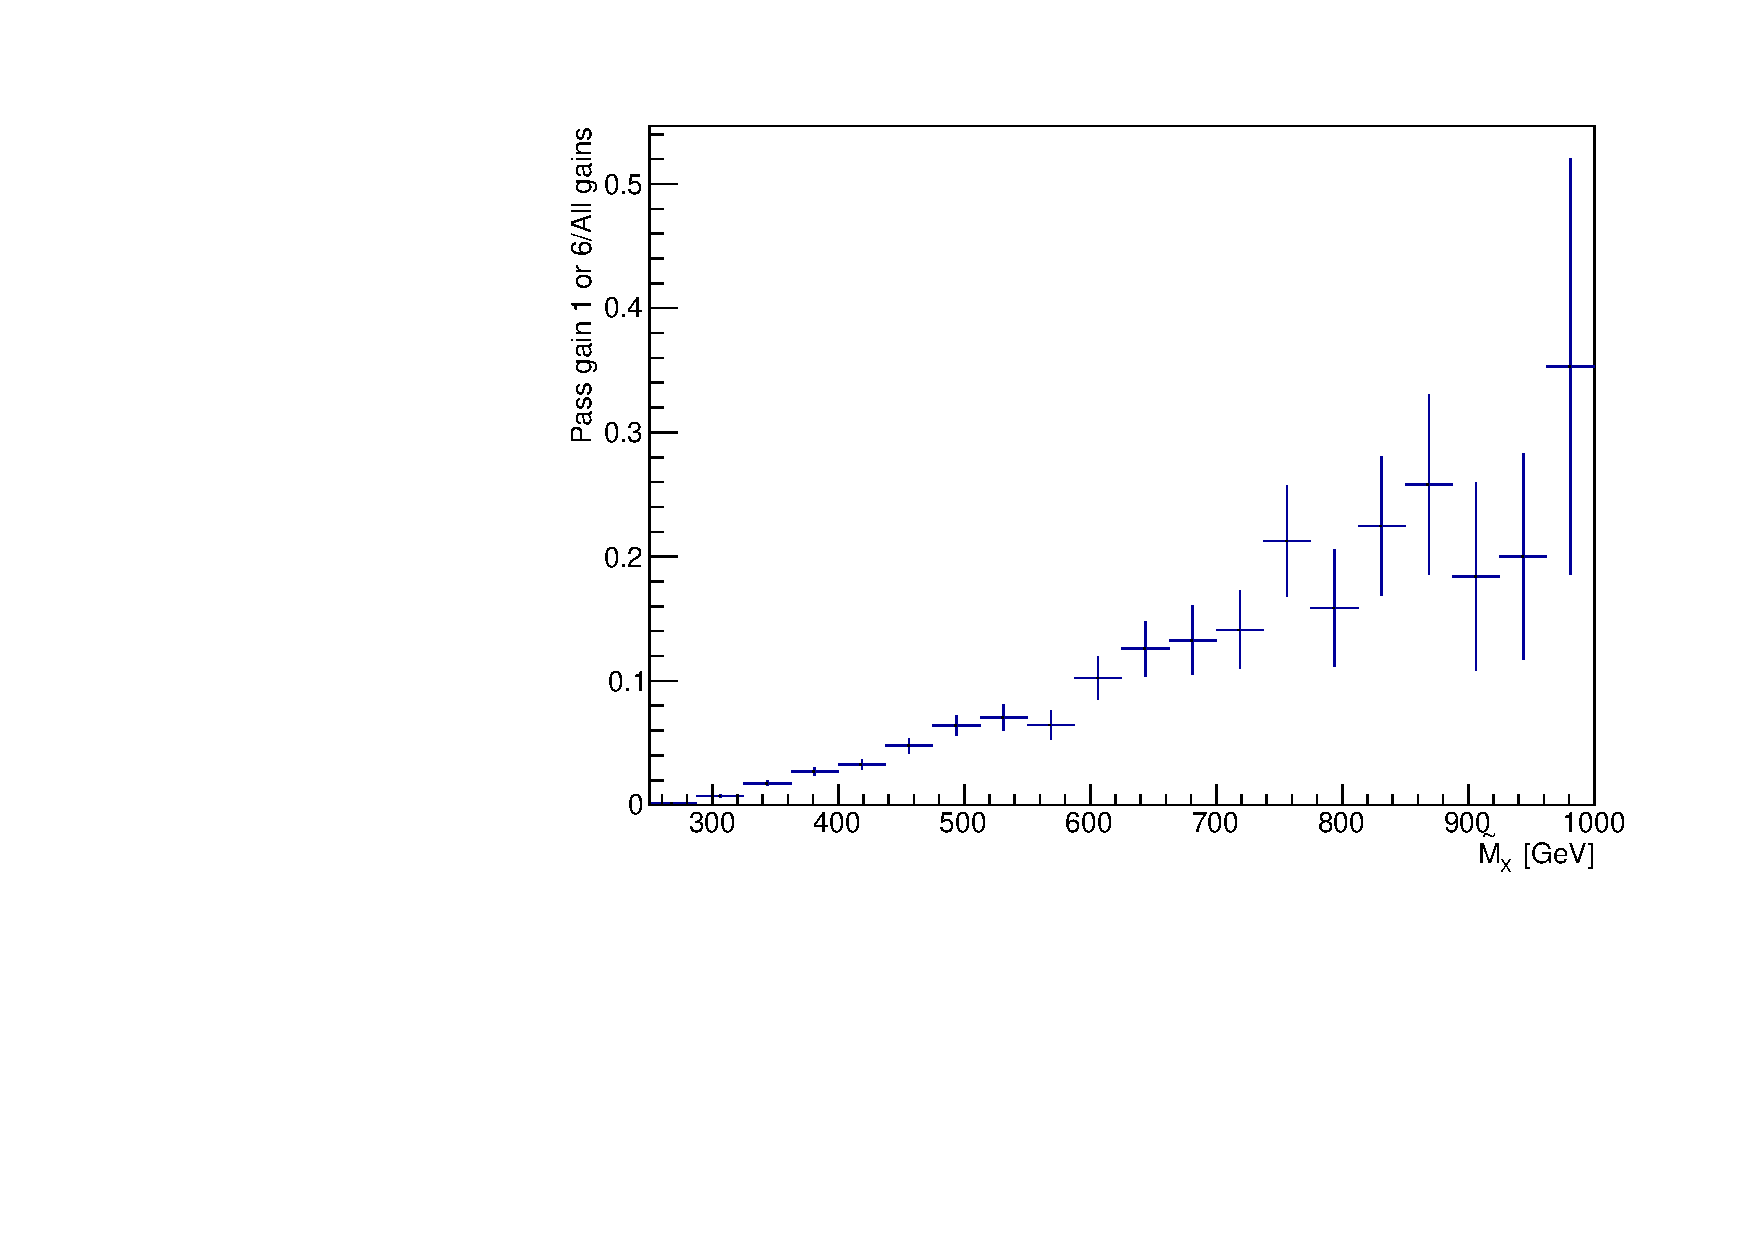
\includegraphics[width=0.3\textwidth]{figures/sec-photons/rg16}\hfil
  \caption{Fraction of events with photon candidates going through gain switch.}
  \label{fig:gain_switch}
\end{figure*}

\subsubsection{Regression}

A new version of the photon energy regression has been trained (with 80X MC and 2016 data taking conditions). 
We compared this new regression to the previous training (74X), as seen in the plots of Figure \ref{fig:pho_reg} for three different resonance mass points. 
The difference observed is not large enough for this analysis to be affected, so the regression version used is 74X (following main $\Hgg$ analysis).

\begin{figure*}[thb]
  \centering
  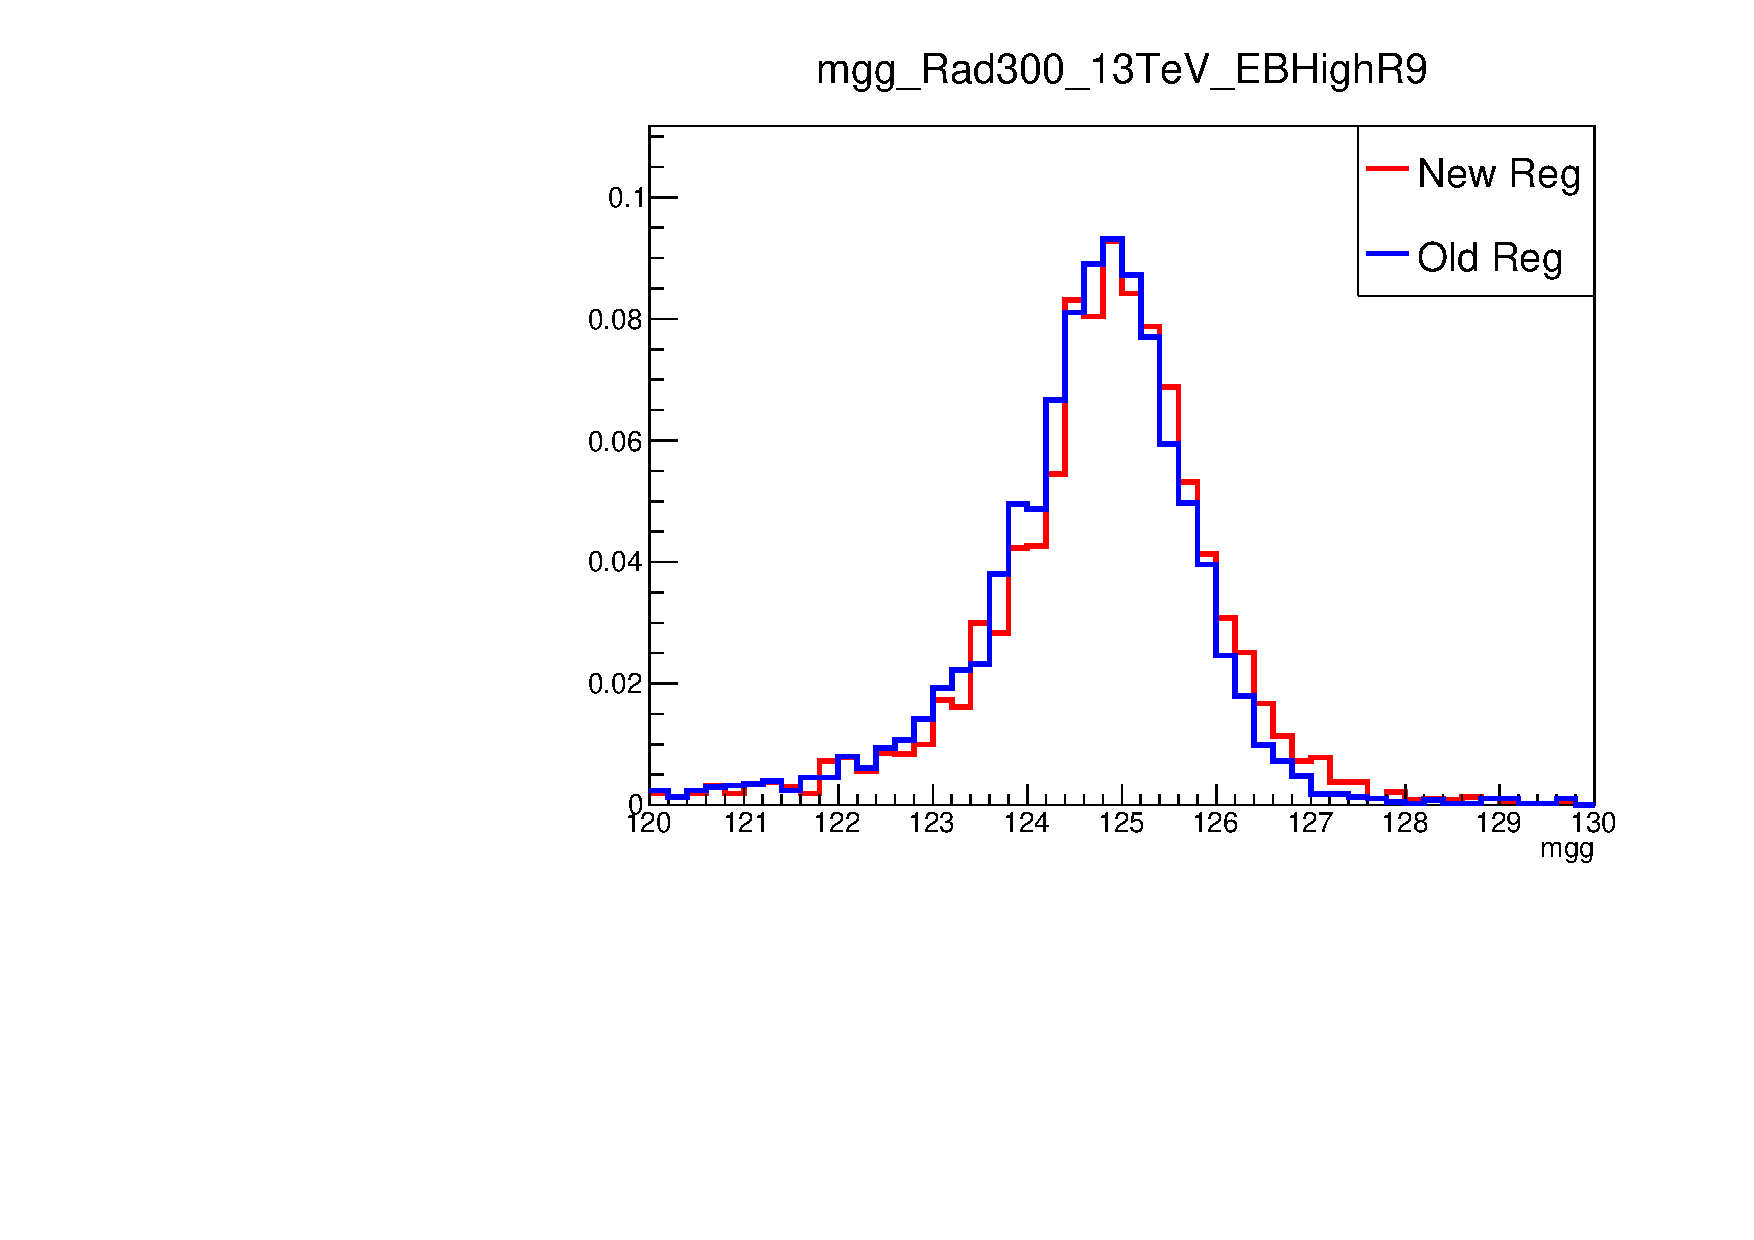
\includegraphics[width=0.3\textwidth]{figures/sec-photons/mgg_Rad300_13TeV_EBHighR9.pdf}\hfil
  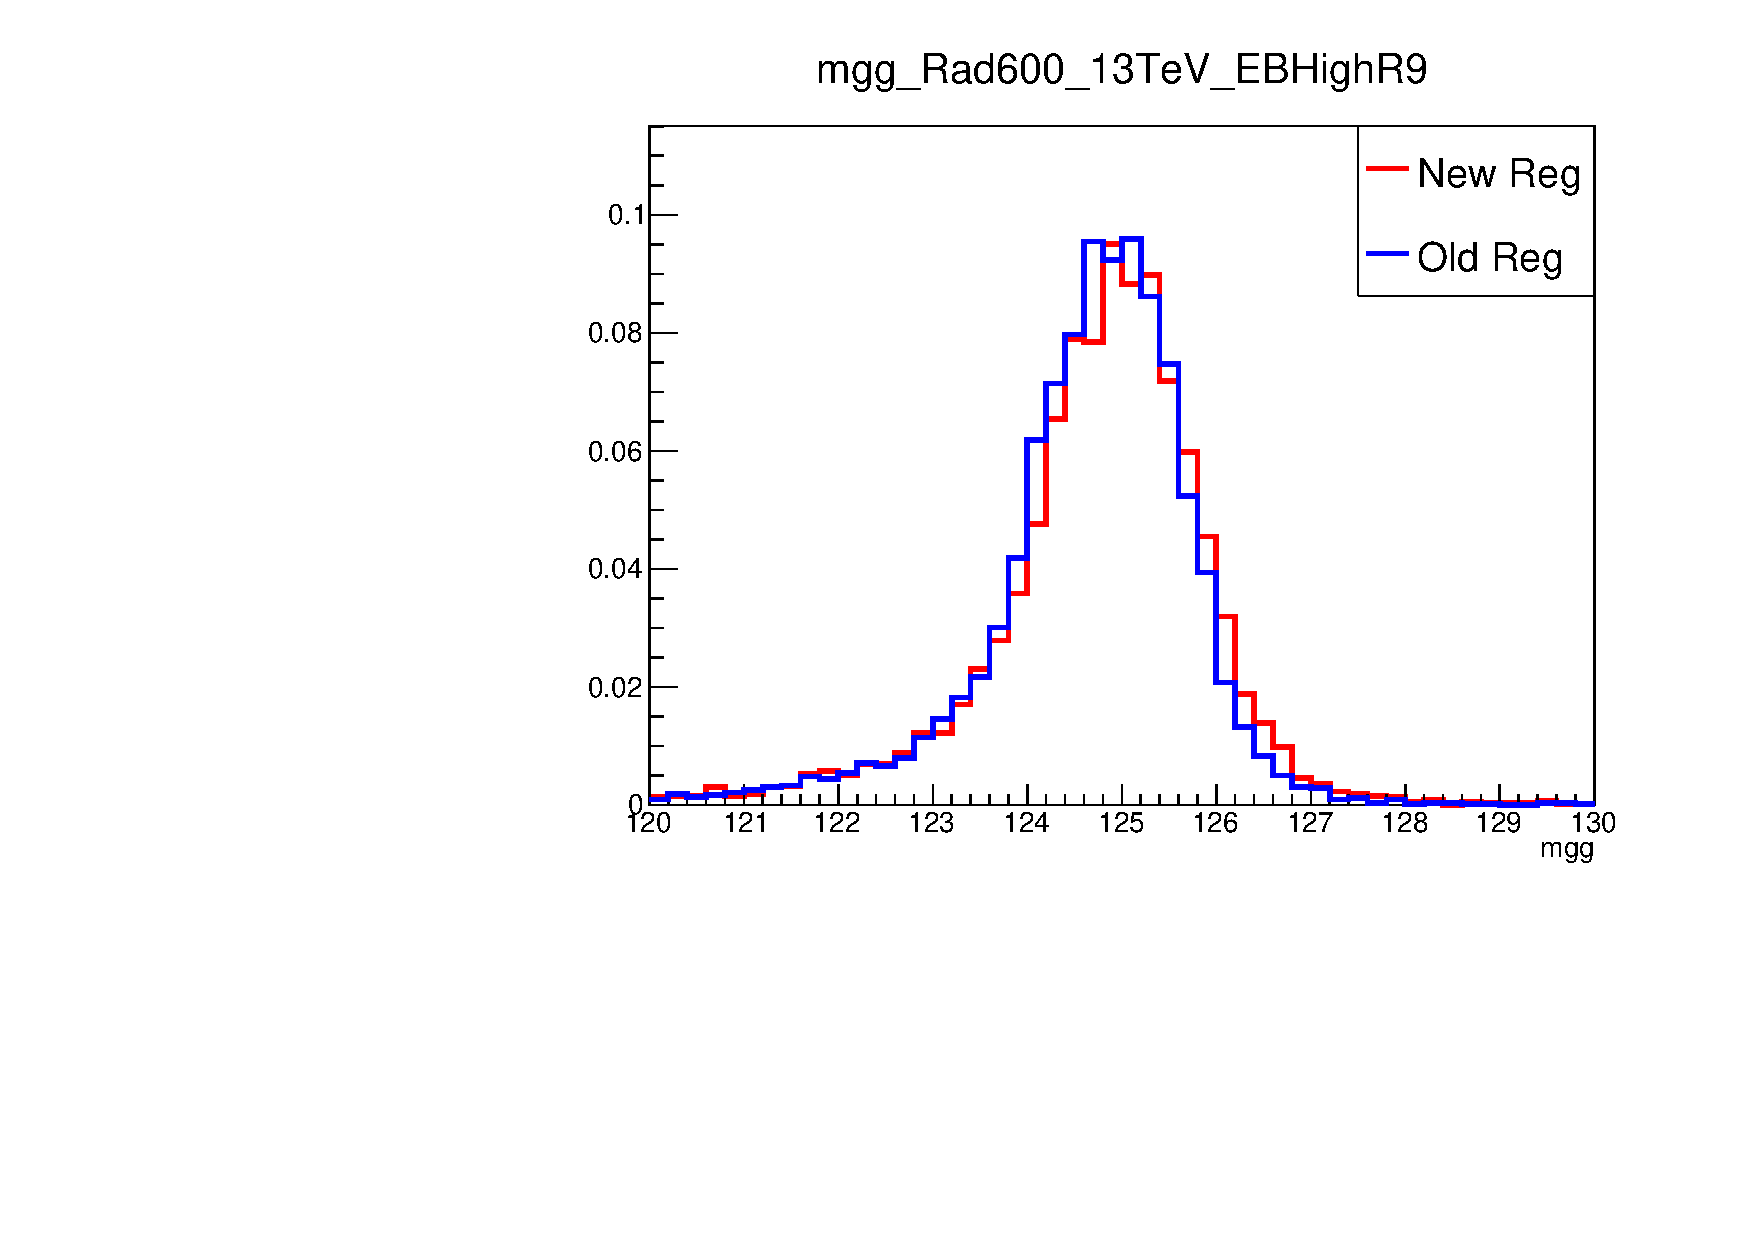
\includegraphics[width=0.3\textwidth]{figures/sec-photons/mgg_Rad600_13TeV_EBHighR9.pdf}\hfil
  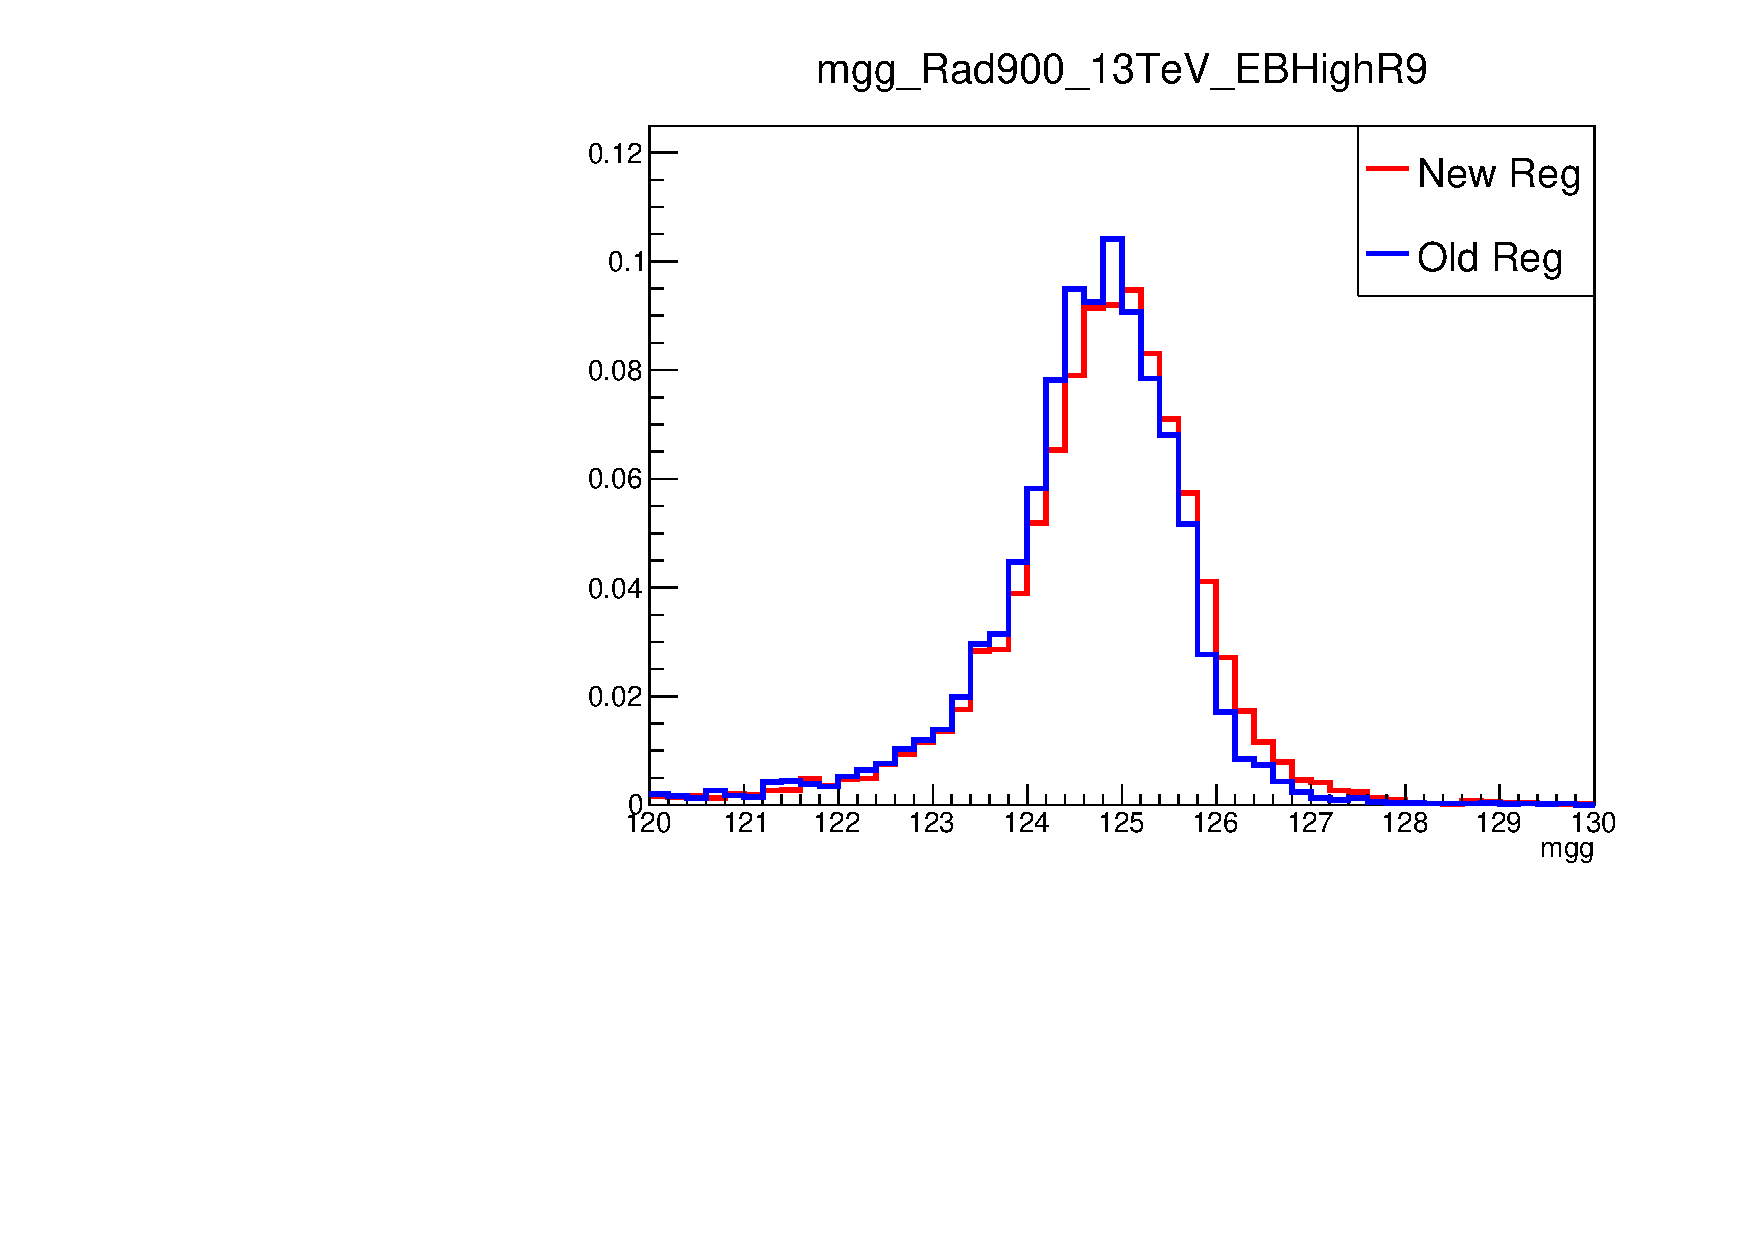
\includegraphics[width=0.3\textwidth]{figures/sec-photons/mgg_Rad900_13TeV_EBHighR9.pdf}\hfil
  \caption{$M(\gamma\gamma)$ reconstructed with different versions of the photon energy regression.}
  \label{fig:pho_reg}
\end{figure*}
